\section{Versuchsanordnung}

\subsection{Versuchsaufbau}

Der Aufbau dieses Versuchs besteht aus 
\begin{figure}[H]
	\centering
	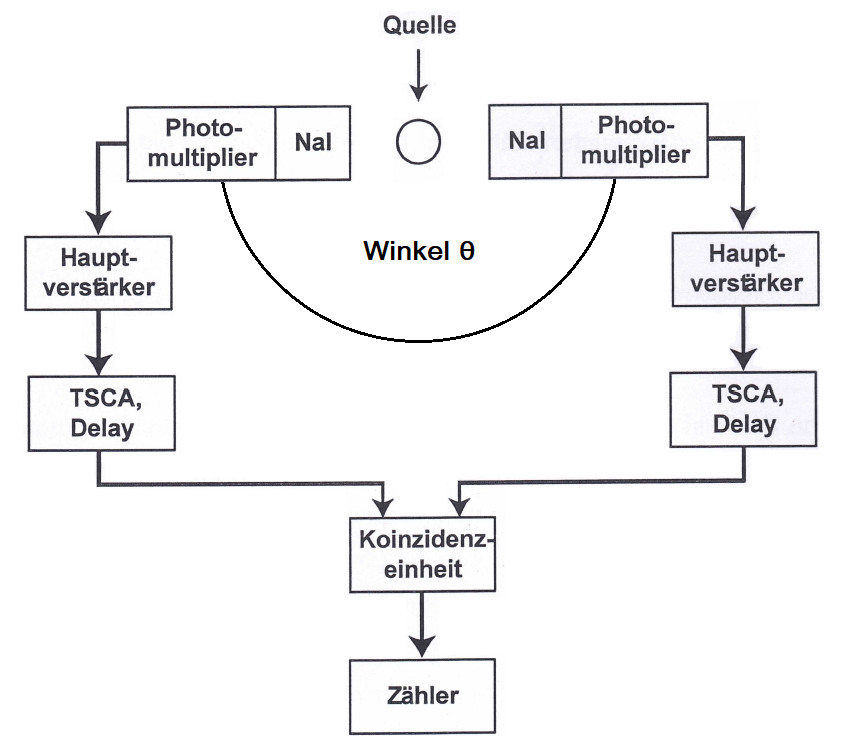
\includegraphics[width=1.0\textwidth]{img/schaltung}
	\caption{Die Abbildung zeigt .}
	\label{schaltung}
\end{figure}
\noindent 

\subsection{Elektronik}


\begin{figure}[H]
	\centering
	\begin{subfigure}[t]{0.495\textwidth}
		\centering
		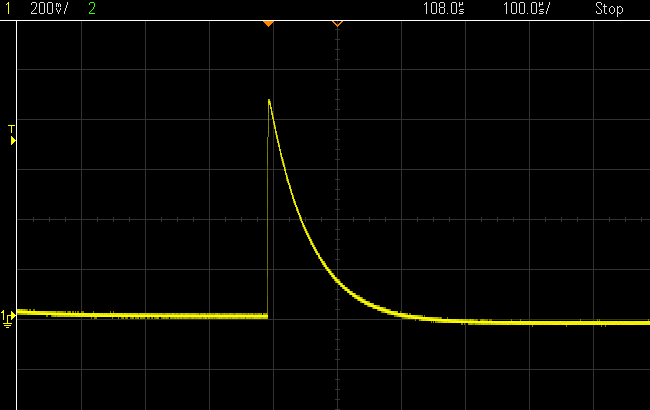
\includegraphics[width=\textwidth]{img/SignalNachPhotomultiplier}
		\caption{Oszilloskopbild des Signals am Photomultiplier.}
		\label{SignalNachPhotomultiplier}
	\end{subfigure}
	\begin{subfigure}[t]{0.495\textwidth}
		\centering
		\includegraphics[width=\textwidth]{img/SignalNachHauptverstärker}
		\caption{Oszilloskopbild des Signals nach dem Hauptverstärker.}
		\label{SignalNachHauptverstärker}
	\end{subfigure}
	\begin{subfigure}[t]{0.495\textwidth}
		\centering
		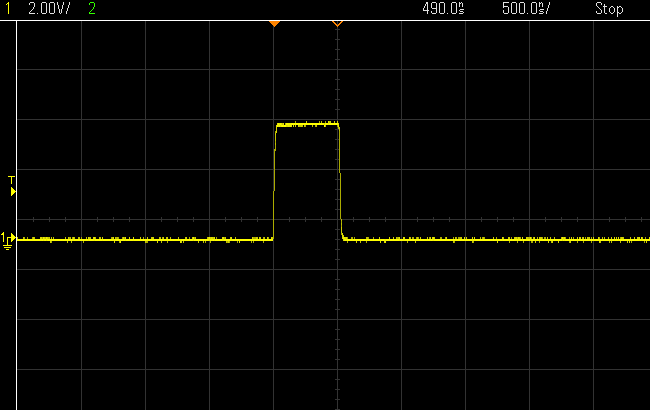
\includegraphics[width=\textwidth]{img/SignalNachTSCA}
		\caption{Oszilloskopbild des Signals nach dem TSCA.}
		\label{SignalNachTSCA}
	\end{subfigure}
	\begin{subfigure}[t]{0.495\textwidth}
		\centering
		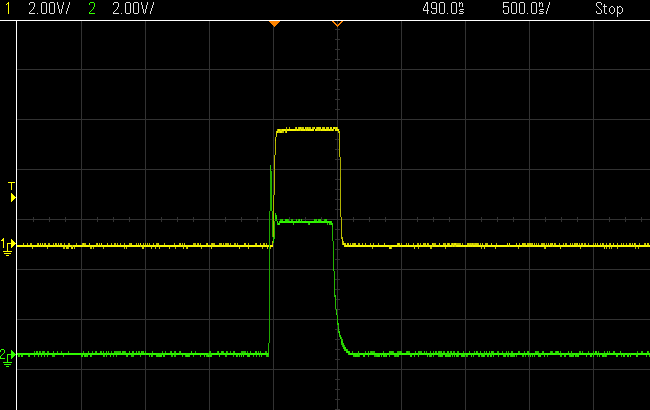
\includegraphics[width=\textwidth]{img/BeideSignaleVorKoinzidenzeinheit}
		\caption{Oszilloskopbild beider aus den TSCA stammenden Signale vor der Koinzidenzeinheit.}
		\label{BeideSignaleVorKoinzidenzeinheit}
	\end{subfigure}
	\caption{Die Abbildung zeigt die mit einem Oszilloskop dargestellten Bilder des Signals.}
	\label{Oszilloskopbilder}
\end{figure}
\noindent 